\documentclass{beamer}

\usepackage[utf8]{inputenc}
\usepackage[serbian]{babel}

\title{Gađanje mete}
\author{Vasilić Marko IN/2019\\ Savković Jovan IN/2019}
\date{}

\usecolortheme{seahorse}


\begin{document}

\frame{\titlepage}

\begin{frame}
	\frametitle{Opis problema}

	\begin{columns}
		\column{0.4\textwidth}
		2D igrica - gađanje mete
		
		Igrač bira projektil kojim gađa metu, ali na polju se nalaze prepreke u vidu debelih i tankih zidova.

		Igrač mora da izabere projektil koji će najbolje obaviti posao. Šuriken će uništiti tanke zidove, lopta će se odbiti od sve zidove. Treba kombinovati projektile tako da se oslobodi put do mete.
		
		\column{0.6\textwidth}
		\fbox{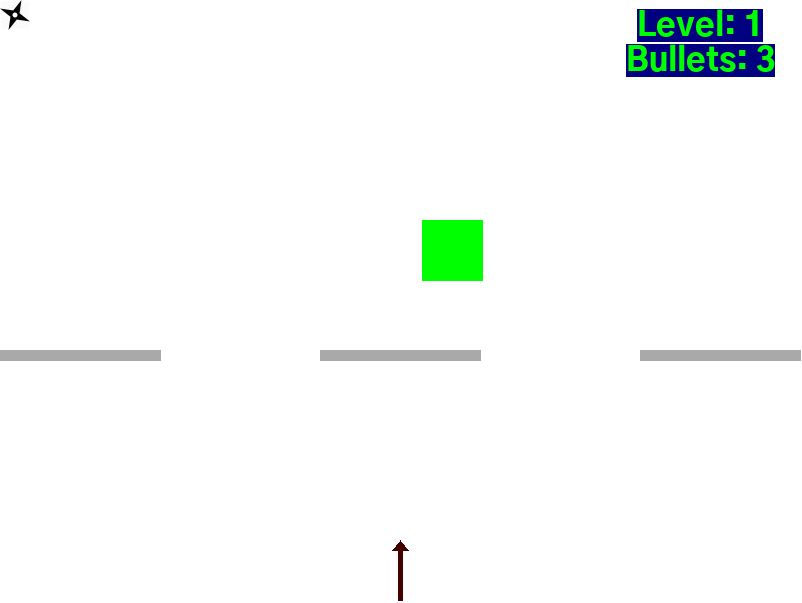
\includegraphics[scale=0.22]{./images/igrica.png}}
	\end{columns}
\end{frame}

\begin{frame}
	\frametitle{Kontrole}
	
	\begin{columns}
		\column{0.4\textwidth}
		\begin{itemize}
			\item Ciljanje:
			\\
			
\includegraphics[scale=0.7]{./images/levo.png}
			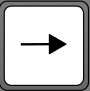
\includegraphics[scale=0.73]{./images/desno.png}
			\item Pucanje:
			
\includegraphics[scale=0.7]{./images/space.png}
			\item Biranje municije:
			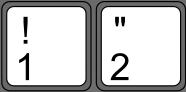
\includegraphics[scale=0.7]{./images/12.png}
			\item Resetovanje igrice:
			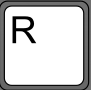
\includegraphics[scale=0.7]{./images/r.png}
			\item Zaustavljanje aktivnog projektila:
			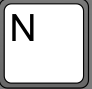
\includegraphics[scale=0.7]{./images/n.png}
		\end{itemize}
		\column{0.6\textwidth}
		\begin{center}
			\fbox{
\includegraphics[scale=0.5]{./images/strelica.png}}
		\end{center}
		\begin{center}
		Strelica za ciljanje
		\end{center}
		\vspace{2cm}
	\end{columns}
\end{frame}

\begin{frame}
	\frametitle{Elementi rešenja}
	\Large
	\begin{itemize}
		\item Kinematika - pravolinijsko kretanje i rotaciono kretanje\\
		\textbf{Rešenje} - RK4
		\item Detekcija kolizije\\
		\textbf{Rešenje} - GJK
	\end{itemize}
\end{frame}

\begin{frame}
	\frametitle{Detekcija kolizije}
	Detekcija kolizije funkcioniše za bilo koju kombinaciju krugova, poligona i duži
	
	Za detekciju kolizije koristi se GJK algoritam.
	\begin{center}
		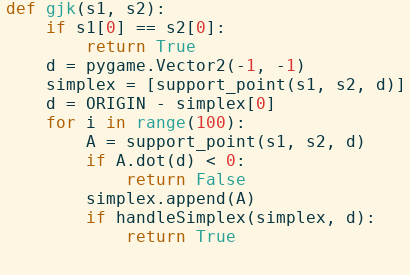
\includegraphics[scale=0.5]{./images/gjk.png}
	\end{center}
\end{frame}

\begin{frame}
	\frametitle{GJK}
	\Large
	Minkowski razlika
	\begin{center}
		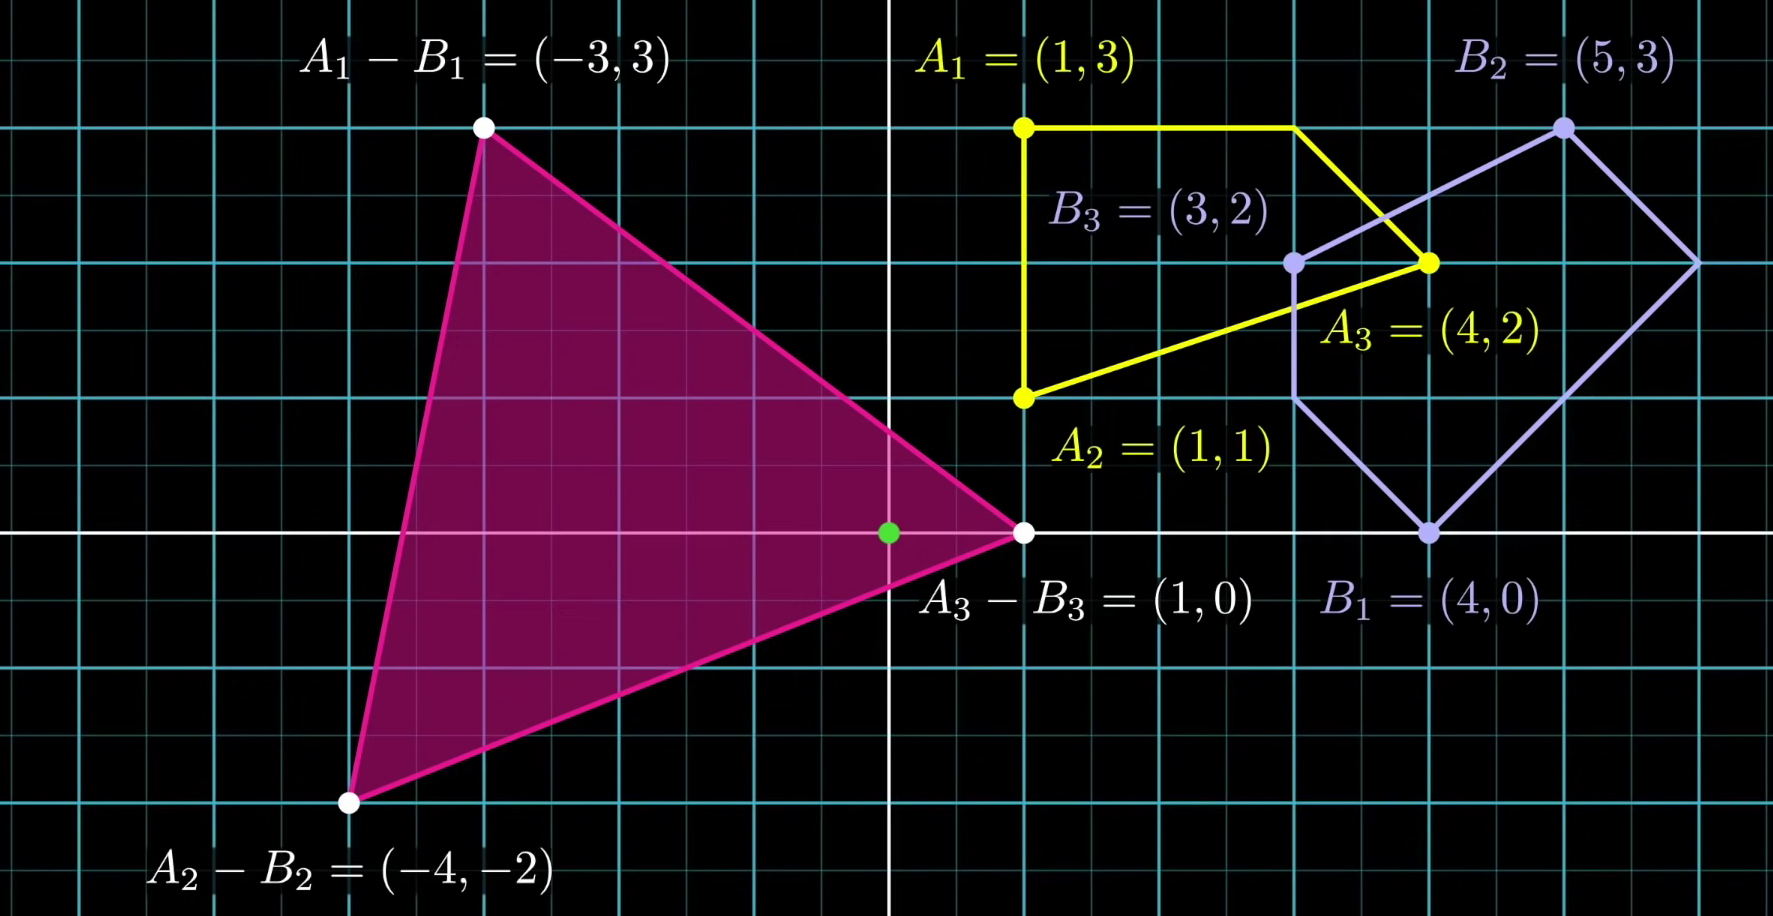
\includegraphics[scale=0.17]{./images/gjk1.png}
	\end{center}
\end{frame}

\begin{frame}
	\frametitle{GJK}
	\Large
	Određivanje support pointa
	\begin{center}
		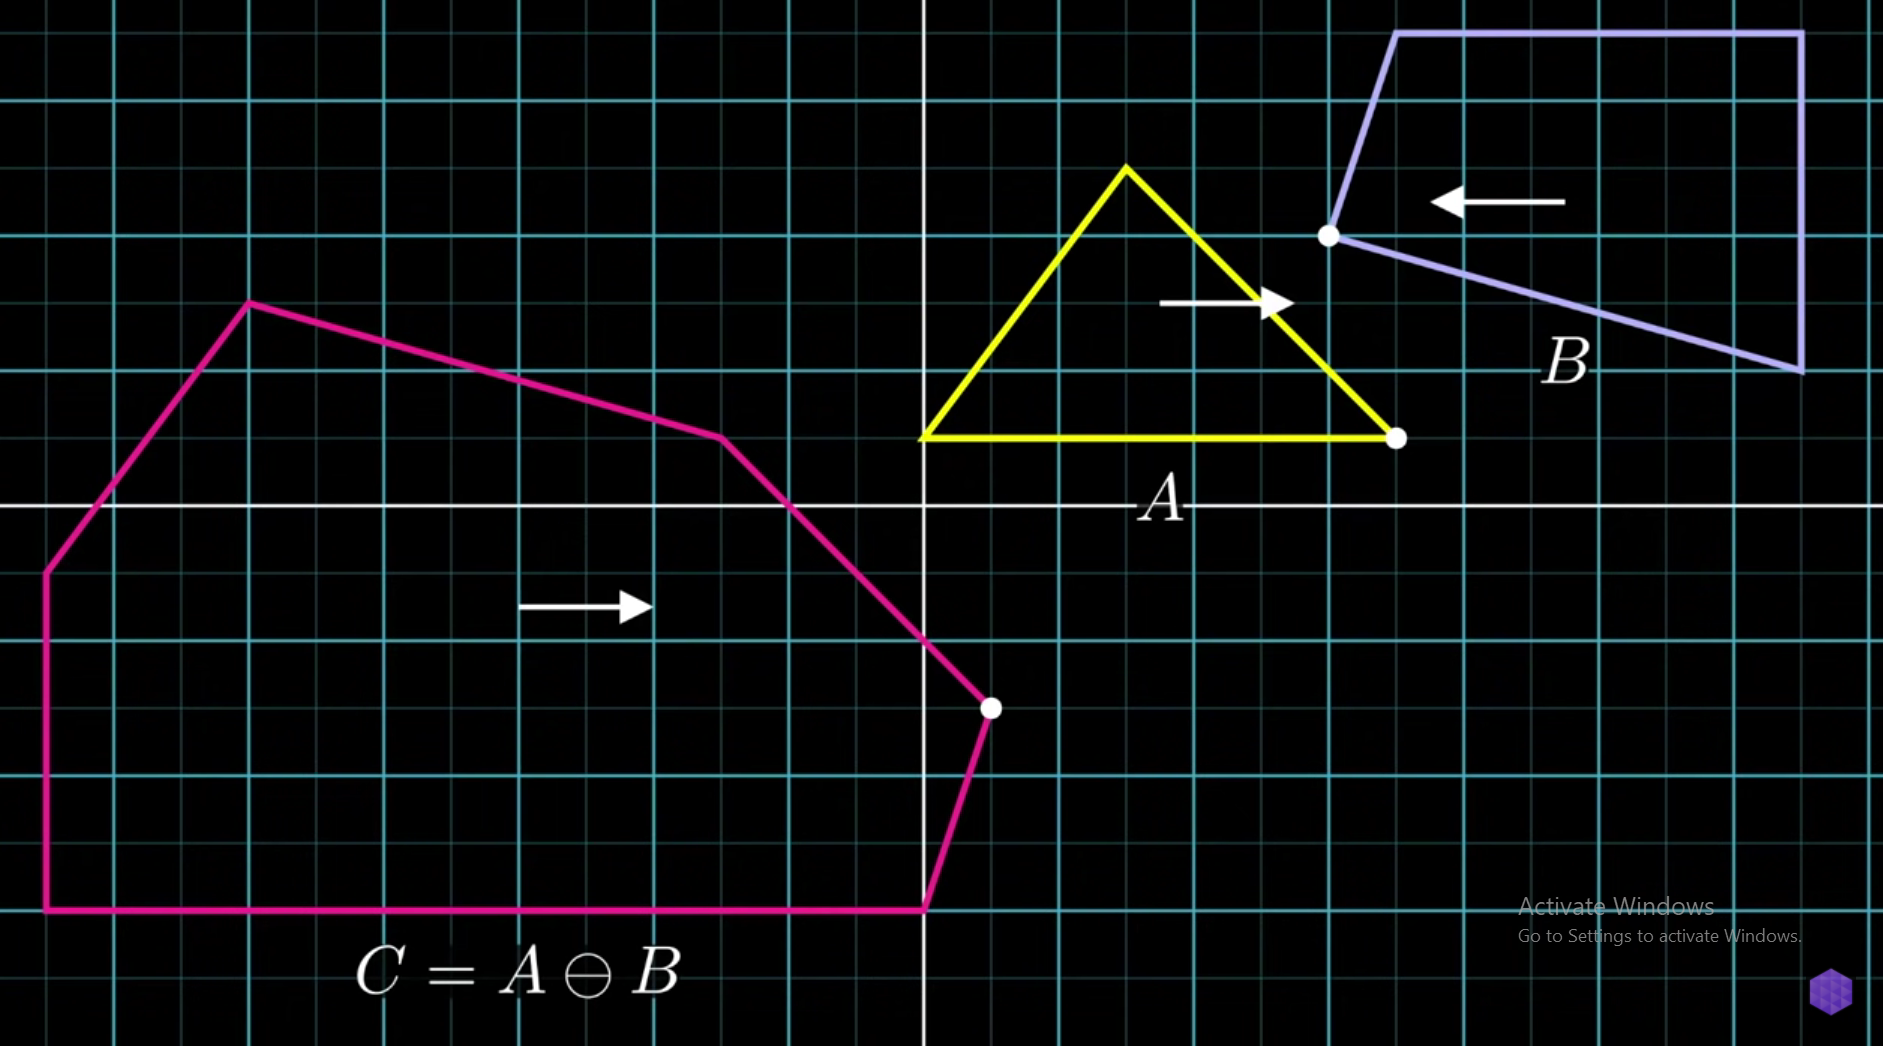
\includegraphics[scale=0.162]{./images/gjk2.png}
	\end{center}
\end{frame}

\begin{frame}
	\frametitle{GJK}
	\Large
	Support point za krug
	\begin{center}
		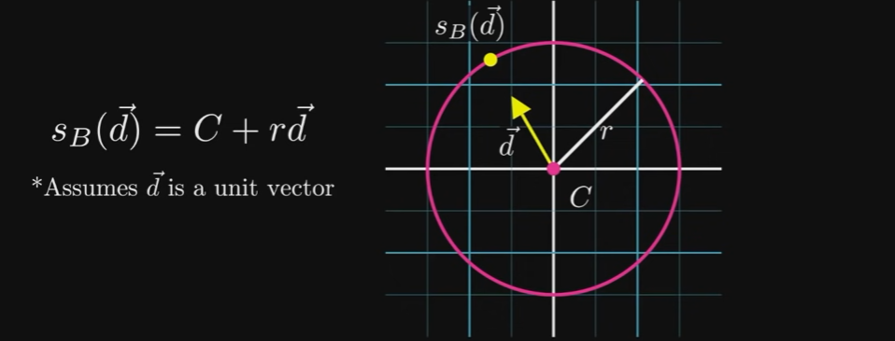
\includegraphics[scale=0.33]{./images/gjk3.png}
	\end{center}
\end{frame}

\begin{frame}
	\frametitle{GJK}
	\Large
	Support point za poligon
	\begin{center}
		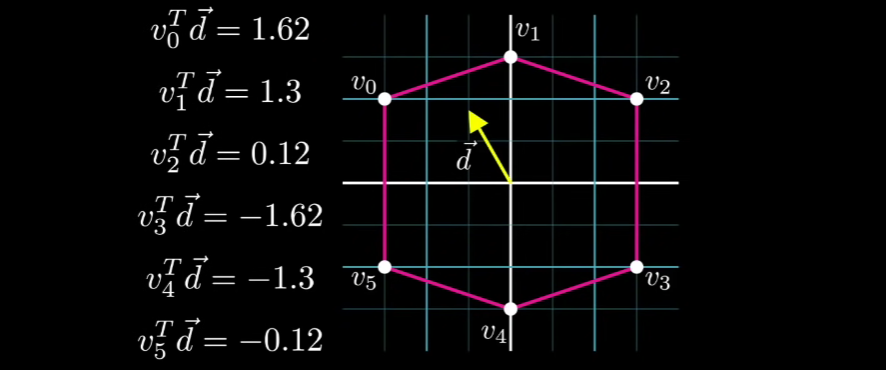
\includegraphics[scale=0.33]{./images/gjk4.png}
	\end{center}
\end{frame}

\begin{frame}
	\frametitle{GJK}
	\Large
	Određivanje vektorskog proizvoda
	\begin{center}
		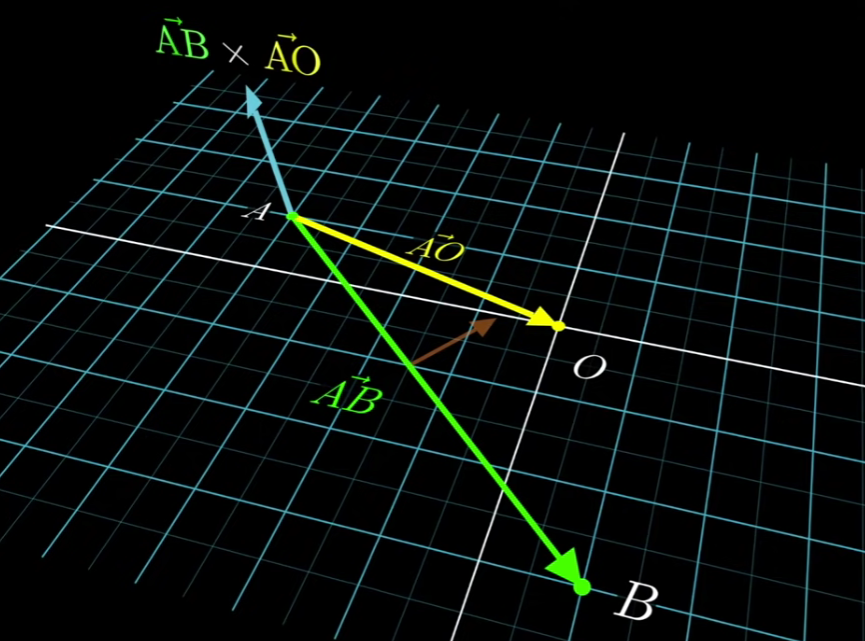
\includegraphics[scale=0.3]{./images/gjk5.png}
	\end{center}
\end{frame}

\begin{frame}
	\frametitle{GJK}
	\begin{columns}
		\column{0.5\textwidth}
		\begin{center}
			\Large
			Uspešno
			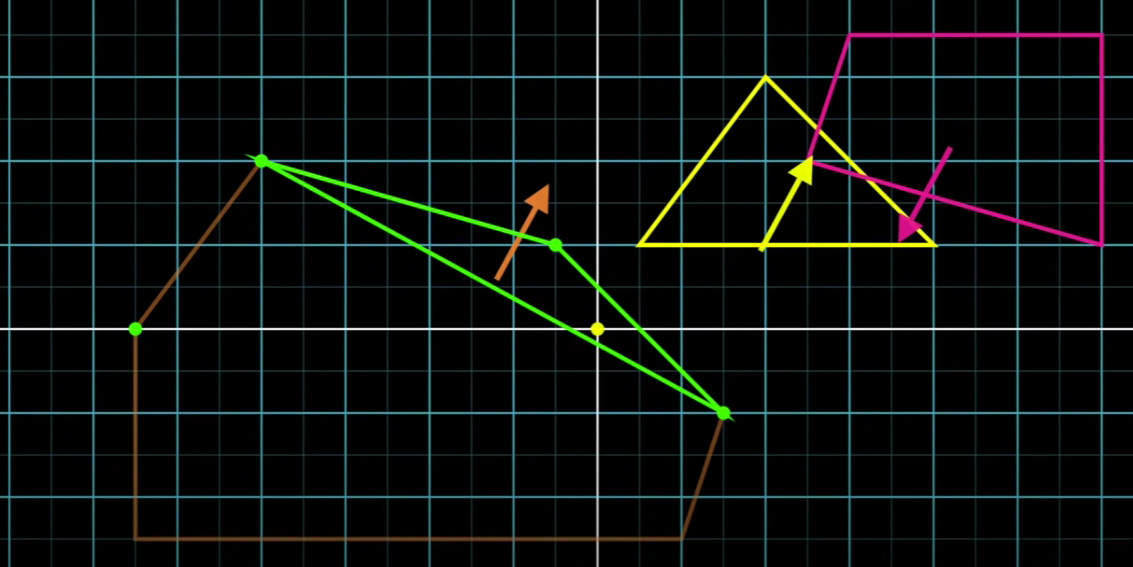
\includegraphics[scale=0.141]{./images/gjk6.png}
		\end{center}
		\column{0.5\textwidth}
		\begin{center}
			\Large
			Neuspešno
			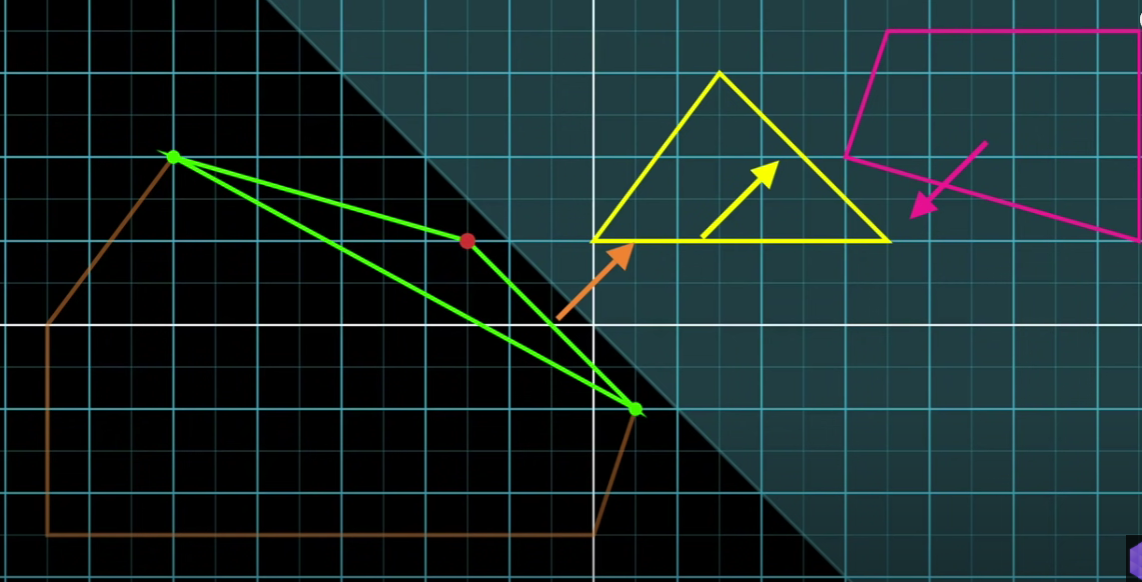
\includegraphics[scale=0.14]{./images/gjk7.png}
		\end{center}
	\end{columns}
\end{frame}

\begin{frame}
	\frametitle{GJK}
	\Large
	Određivanje da li trougao sadrži koordinatni početak
	\begin{center}
		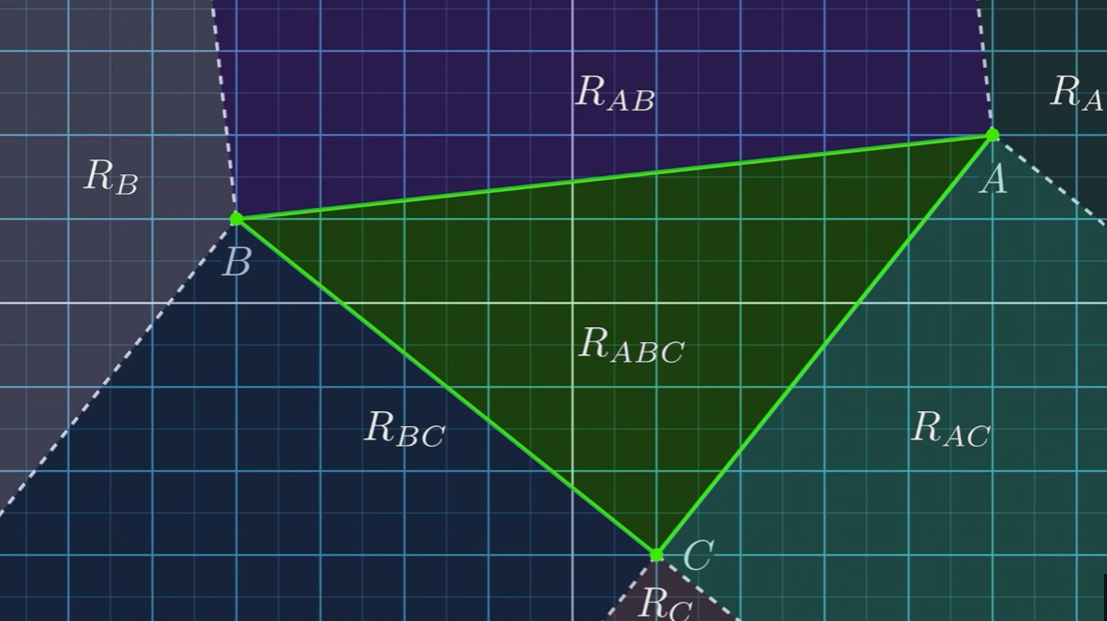
\includegraphics[scale=0.26]{./images/gjk8.png}
	\end{center}
\end{frame}

\begin{frame}
	\frametitle{Odbijanje o zidove}
	Projektil "lopta" će se odbiti od zidove.
	
	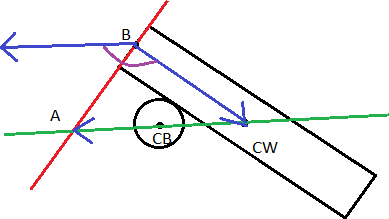
\includegraphics[scale=0.75]{./images/odbijanje3.png}
\end{frame}

\begin{frame}
	\frametitle{Odbijanje o zidove}
	
	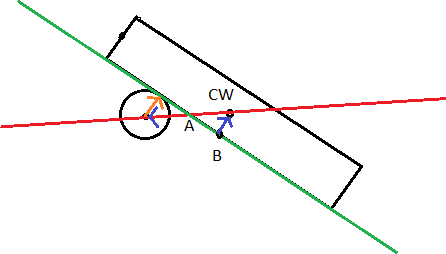
\includegraphics[scale=0.67]{./images/odbijanje2.png}
\end{frame}

\begin{frame}
	\frametitle{Odbijanje o zidove}
	
	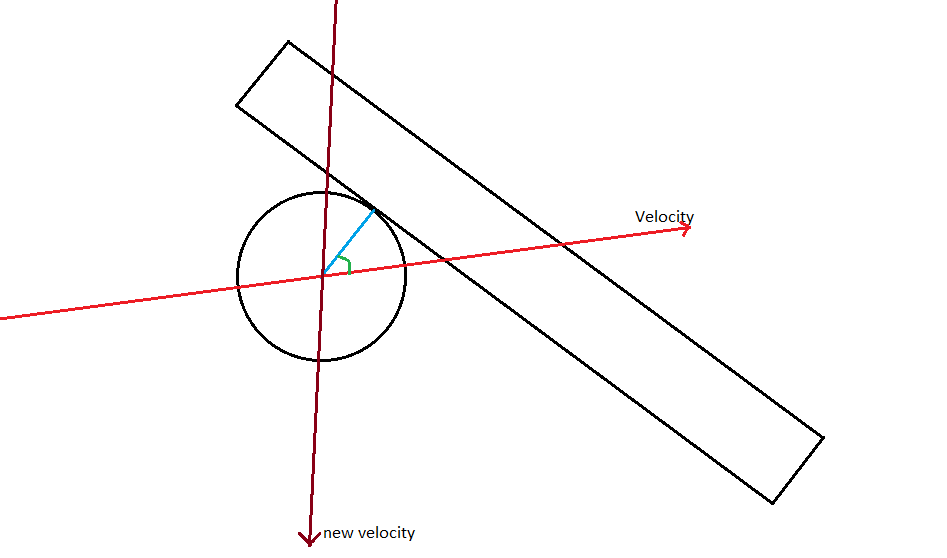
\includegraphics[scale=0.34]{./images/odbijanje1.png}
\end{frame}

\begin{frame}
	\frametitle{Detekcija kolizije - šuriken}
	Šuriken nije konveksan poligon, tako da gjk ne bi radio za njega.

	Ovaj problem je rešen tako što se šuriken posmatra kao skup 4 konveksna poligona. U koliko se detektuje kolizija sa bilo kojim od poligona koji ga sačinjavaju, smatra se da je šuriken došao u kontakt sa nečim.
	
	\vspace{0.4cm}
	\begin{center}
		
\includegraphics[scale=0.3]{./images/shuriken.png}
	\end{center}
\end{frame}

\begin{frame}
	\frametitle{Kinematika}
	Pravolinijsko i rotaciono kretanje je pretstavljeno kao diferencijalna jednačina.
	
	Pomoću RK4 algoritma se aproksimira vrednost datih funkcija kretanja pri svakom koraku igrice.
	
	\vspace{0.8cm}
	\begin{center}
		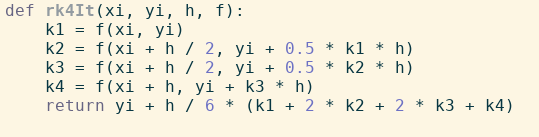
\includegraphics[scale=0.5]{./images/rk4.png}
	\end{center}
\end{frame}

\begin{frame}
	\frametitle{RK4}
	\begin{center}
		Pravolinijsko kretanje
		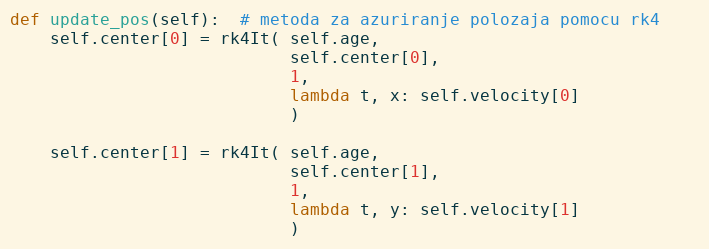
\includegraphics[scale=0.3]{./images/rk4pos.png}
		
		\vspace{0.3cm}
		Rotaciono kretanje
		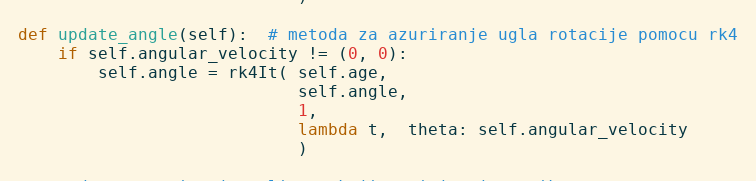
\includegraphics[scale=0.3]{./images/rk4angle.png}
	\end{center}
\end{frame}

\begin{frame}
	\frametitle{Nivoi}
	\Large
	Igrica se sastoji od 3 novoa koji služe da demonstriraju funkcionalnosti igre.
	
	Za svaki nivo igrač ima na raspolaganju 3 projektila da pogodi metu, u koliko ne pogodi kreće ispočetka.
\end{frame}

\begin{frame}
	\frametitle{Nivo 1}
	\Large
	Jednostavno gađanje mete.
	
	\vspace{0.5cm}
	
	\begin{center}
		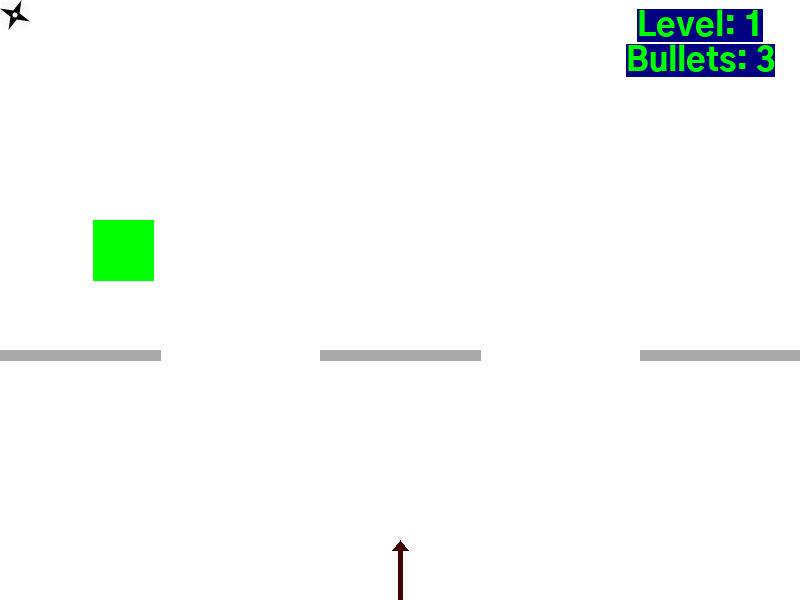
\includegraphics[scale=0.25]{./images/lvl1.png}
	\end{center}
\end{frame}
\begin{frame}
	\frametitle{Nivo 2}
	\Large
	Igrač mora prvo da pomoću šurikena uništi jedan od tankih zidova, zatim da pogodi metu proizvoljnim projektilom.
	
	\vspace{0.5cm}
	
	\begin{center}
		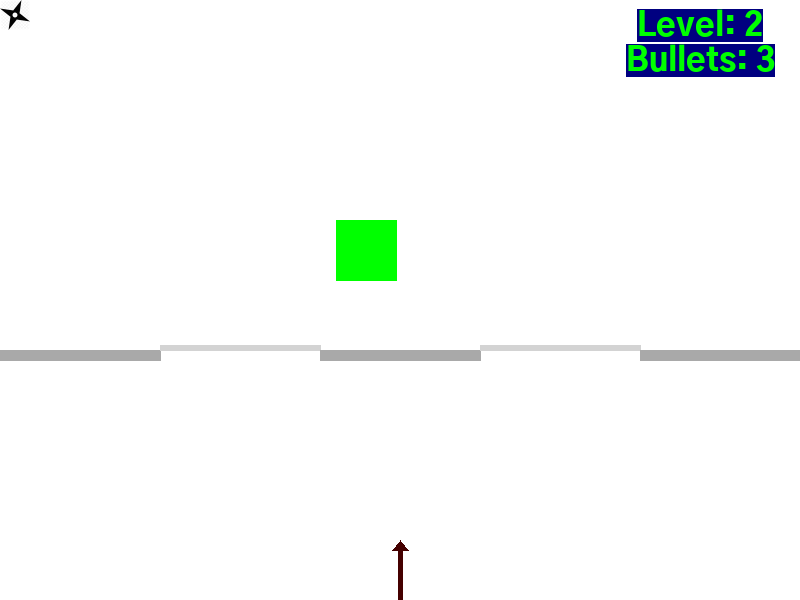
\includegraphics[scale=0.25]{./images/lvl2.png}
	\end{center}
\end{frame}
\begin{frame}
	\frametitle{Nivo 3}
	\Large
	Igrač mora da odbije lopticu od dijagonalni zid na desnoj strani ekrana da bi pogodio metu.
	
	\vspace{0.5cm}
	
	\begin{center}
		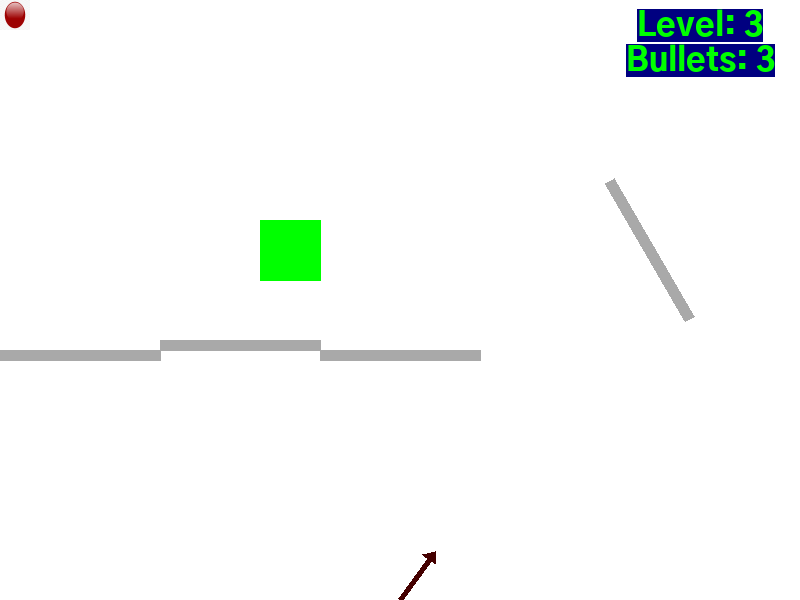
\includegraphics[scale=0.25]{./images/lvl3.png}
	\end{center}
\end{frame}
\begin{frame}
	\begin{center}
		\Huge
		\textbf{Hvala na pažnji}
	\end{center}
\end{frame}
\end{document}
